\section{Appendix}
%\section{Appendix: Experimental Findings}
\label{app:app}
% SAC 2027: all tables and figures that the text relies on were moved into the
% main body; the appendix keeps only the photo of the test bench.







\begin{figure}[!htbp]
    \centering
    \includegraphics[width=1\linewidth]{fig/devices.jpeg}
    \caption{Controlled experiment devices.}
    \Description{Photograph of the test bench on a desk: an Apple TV, a Fire TV stick with its remote, a HomePod mini, the D-Link, Eufy, Reolink, Tapo C100, Tapo C200, and Xiaomi cameras, and the Raspberry Pi used as the access point, each labelled with its name.}
    \label{fig:devices}
\end{figure}



%% Devices used











%% %% 
%% 





%Abbreviation for update service provider in the above table

%National Institute of Standards and Technology (NIST), University of Colorado (CU), Japan Network Information Center (JNIC),  Vetta Online Ltd (VO),
%FDCservers.net LLC (FDC),
%Aussie Broadband (AB),
%Aliyun Computing Co. Ltd, 
% Chunghwa Telecom Co. Ltd.
%%%%%%%%%
%%%%%%%%


% Update providers

%\textbf{Update supplier:}



%%%%%%%%%
%%%%%%%%









%\textbf{Protocols used:}
%% After removing artifcats and non- related protocols



%%%%%%%
%%%%%%%



























%% Retrospective counterpart of Figure~\ref{fig:entropy_heatmap} (\S\ref{sec:results}).



%% Per-payload entropy distributions, both experiments (moved here from \S\ref{sec:results}).







\begin{comment}
    
\textbf{Security bits distribution:}
Figure~\ref{fig:security_bits_boxplot_all} presents the distribution of security bits across devices with NIST reference thresholds.
The majority of certificates cluster at 112 bits (RSA-2048), with the NIST 128-bit minimum clearly separating strong from transitional deployments.
Tapo-c100 shows the widest spread due to its mix of broken (80-bit) and weak (112-bit) certificates, resulting in the lowest average security strength of 69.3 bits among all devices.
\end{comment}


%% Cipher-suite classification criteria + adversarial capability (addresses formalization request)
%% Cipher-suite classification criteria + adversarial capability (addresses formalization request)












%\textbf{Contacted countries:}










% BLIND REVIEW: the camera frame in these screenshots shows a person; crop or
% blur it before restoring in a blind submission.
% [SAC 2027 page limit] Not cited in the text; excluded so the paper stays within
% the 10-page maximum. Delete this comment/endcomment pair to restore it.
\begin{comment}
\begin{figure}
    \centering
    \begin{subfigure}[b]{0.32\linewidth}
        \centering
        \includegraphics[width=\linewidth]{fig/riolink_uploading.png}
        \caption{Uploading}
        \label{fig:riolink_uploading}
    \end{subfigure}
    \hfill
    \begin{subfigure}[b]{0.32\linewidth}
        \centering
        \includegraphics[width=\linewidth]{fig/riolink_updating.png}
        \caption{Updating}
        \label{fig:riolink_updating}
    \end{subfigure}
    \hfill
    \begin{subfigure}[b]{0.32\linewidth}
        \centering
        \includegraphics[width=\linewidth]{fig/riolink_updated.png}
        \caption{Completed}
        \label{fig:riolink_updated}
    \end{subfigure}
    \caption{Reolink firmware update process.}
    \Description{Three screenshots of the Reolink desktop client: a firmware-update dialog stating that the device is upgrading while the file uploads, the same dialog with the upgrade progress bar, and an update-completed message.}
    \label{fig:riolink_update_process}
\end{figure}
\end{comment}









% [SAC 2027 page limit] Not cited in the text; excluded so the paper stays within
% the 10-page maximum. Delete this comment/endcomment pair to restore it.
\begin{comment}
\begin{figure}[htbp]
    \centering
    \begin{subfigure}[b]{0.48\linewidth}
        \centering
        \includegraphics[width=\linewidth]{fig/apple-tv.jpeg}
        \caption{Update checking}
        \label{fig:apple-tv_checking}
    \end{subfigure}
    \hfill
    \begin{subfigure}[b]{0.48\linewidth}
        \centering
        \includegraphics[width=\linewidth]{fig/apple-tv1.jpeg}
        \caption{Update Downloading}
        \label{fig:apple-tv_downloading}
    \end{subfigure}
    \caption{Apple TV update.}
    \Description{Two photographs of the Apple TV Software Updates screen: a dialog offering the tvOS 26.2 update with download-and-install and later buttons, and a progress bar for the download with about eight minutes remaining.}
    \label{fig:apple_update}
\end{figure}
\end{comment}














%% Certifictate key sizes











%% 






%% %% 
%%  CWE




























































%\begin{figure}
 %   \centering
    %\includegraphics[width=0.9\linewidth]{fig/device_comparison_key_size.pdf}
    %\caption{Per-device comparison of certificate key sizes.}
    %\label{fig:device_comparison_key_size}
%\end{figure}



%\begin{figure}[htbp]
 %   \centering
  %  \includegraphics[width=0.9\linewidth]{fig/device_comparison_strength.pdf}
   % \caption{Per-device certificate strength classification following NIST SP~800-57 guidelines.}
    %\label{fig:device_comparison_strength}
%\end{figure}



%\textbf{Note for now:}
%d-link-cam is already up to date; however, we trigger an update and notice that the device is using  Simple Service Discovery Protocol (SSDP) and provide two info; SEARCH  and SEARCH through *HTTP/1.1.
%Also the sony-tv and fire-tv-stick devices are uptodate.














%\section{Figures from the experiments}















% [SAC 2027 page limit] Not cited in the text; excluded so the paper stays within
% the 10-page maximum. Delete this comment/endcomment pair to restore it.
\begin{comment}
\begin{figure}[htbp]
    \centering

    
    \begin{subfigure}[b]{0.3\linewidth} \centering
        \includegraphics[width=\linewidth]{fig/tapo1_info.png}
        \caption{Information} \label{fig:tapo1_info}
    \end{subfigure}
    \begin{subfigure}[b]{0.3\linewidth} \centering
        \includegraphics[width=\linewidth]{fig/tapo1_updating.png}
        \caption{Updating} \label{fig:tapo_c1_updating}
    \end{subfigure}  
    \begin{subfigure}[b]{0.3\linewidth} \centering
        \includegraphics[width=\linewidth]{fig/tapo1_updated.png}
        \caption{Updated} \label{fig:tapo_c1_updated}
    \end{subfigure}


    
    \caption{Tapo c1 update process}
    \Description{Three smartphone screenshots of the Tapo app for the Tapo C100: the device settings page with the firmware update entry, the new-firmware-available page while updating, and the firmware-up-to-date page showing version 1.4.3.}
    \label{fig:tapo_c1_update}
\end{figure}
\end{comment}



% [SAC 2027 page limit] Not cited in the text; excluded so the paper stays within
% the 10-page maximum. Delete this comment/endcomment pair to restore it.
\begin{comment}
\begin{figure}[htbp]
    \centering

    
    \begin{subfigure}[b]{0.3\linewidth} \centering
        \includegraphics[width=\linewidth]{fig/tapo_info.PNG}
        \caption{tapo information} \label{fig:tapo_c2_info}
    \end{subfigure}
    \begin{subfigure}[b]{0.3\linewidth} \centering
        \includegraphics[width=\linewidth]{fig/tapo_updating.PNG}
        \caption{tapo updating} \label{fig:tapo_c2_updating}
    \end{subfigure}  
    \begin{subfigure}[b]{0.3\linewidth} \centering
        \includegraphics[width=\linewidth]{fig/tapo_updated.PNG}
        \caption{tapo updated} \label{fig:tapo_c2_updated}
    \end{subfigure}


    
    \caption{Tapo C200 update process}
    \Description{Three smartphone screenshots of the Tapo app for the Tapo C200: the device information page listing firmware version 1.0.10, the new-firmware-available page for version 1.3.16 while updating, and the firmware-up-to-date page.}
    \label{fig:tapo_c2_update}
\end{figure}
\end{comment}













% [SAC 2027 page limit] Not cited in the text; excluded so the paper stays within
% the 10-page maximum. Delete this comment/endcomment pair to restore it.
\begin{comment}
\begin{figure}[htbp]
    \centering

    
    \begin{subfigure}[b]{0.3\linewidth} \centering
        \includegraphics[width=\linewidth]{fig/xiaomi_down.PNG}
        \caption{Downloading} \label{fig:xiaomi_downloading}
    \end{subfigure}
    \begin{subfigure}[b]{0.3\linewidth} \centering
        \includegraphics[width=\linewidth]{fig/xiaomi_install.PNG}
        \caption{Updating} \label{fig:xiaomi_updating}
    \end{subfigure}  
    \begin{subfigure}[b]{0.3\linewidth} \centering
        \includegraphics[width=\linewidth]{fig/xiaomi_updated.PNG}
        \caption{Updated} \label{fig:xiaomi_updated}
    \end{subfigure}


    
    \caption{xiaomi   process}
    \Description{Three smartphone screenshots of the Xiaomi camera firmware update: downloading at zero percent with latest version 4.0.9, installing, and updated successfully.}
    \label{fig:update_xiaomi}
\end{figure}
\end{comment}







% [SAC 2027 page limit] Not cited in the text; excluded so the paper stays within
% the 10-page maximum. Delete this comment/endcomment pair to restore it.
\begin{comment}
\begin{figure}[htbp]
    \centering

    
    \begin{subfigure}[b]{0.3\linewidth} \centering
        \includegraphics[width=\linewidth]{fig/eufi_info.PNG}
        \caption{Information} \label{fig:eufy_information}
    \end{subfigure}
    \begin{subfigure}[b]{0.3\linewidth} \centering
        \includegraphics[width=\linewidth]{fig/eufi_downloading.PNG}
        \caption{Updating ($\approx3m$)} \label{fig:eufy_updating}
    \end{subfigure}  
    \begin{subfigure}[b]{0.3\linewidth} \centering
        \includegraphics[width=\linewidth]{fig/eufi_failed.PNG}
        \caption{Failed} \label{fig:eufi_failed}
    \end{subfigure}


    
    \caption{Eufy   process.}
    \Description{Three smartphone screenshots of the Eufy Indoor Cam Pan and Tilt firmware update: update available for version 2.3.1.6, updating at 78 percent with about three minutes left, and an update-failed message with a retry button.}
    \label{fig:update_eufi}
\end{figure}
\end{comment}










%\begin{figure}
 %   \centering
  %  \includegraphics[width=0.9\linewidth]{fig/IMG_8101.png}
   % \caption{Riolink setup}
   % \label{fig:placeholder}
%\end{figure}









% BLIND REVIEW: these screenshots show the Swedish room name "Vardagsrum" and the
% HomePod serial number; crop or blur them before restoring in a blind submission.
% [SAC 2027 page limit] Not cited in the text; excluded so the paper stays within
% the 10-page maximum. Delete this comment/endcomment pair to restore it.
\begin{comment}
\begin{figure}[htbp]
    \centering

    
    \begin{subfigure}[b]{0.3\linewidth} \centering
        \includegraphics[width=\linewidth]{fig/homepod_info.png}
        \caption{Information} \label{fig:homepod_info}
    \end{subfigure}
    \begin{subfigure}[b]{0.3\linewidth} \centering
        \includegraphics[width=\linewidth]{fig/homepod_update.png}
        \caption{Update} \label{fig:homepod_update}
    \end{subfigure}  
    \begin{subfigure}[b]{0.3\linewidth} \centering
        \includegraphics[width=\linewidth]{fig/homepod_updating.png}
        \caption{Updating} \label{fig:omepod_updating}
    \end{subfigure}


    
    \caption{Homepod mini.}
    \Description{Three smartphone screenshots of the Apple Home app for a HomePod mini: the accessory page with an update-available notice, the update details, and the download in progress.}
    \label{fig:homepod_mini}
\end{figure}
\end{comment}







%\begin{figure}[h]
\centering
\scalebox{1}{
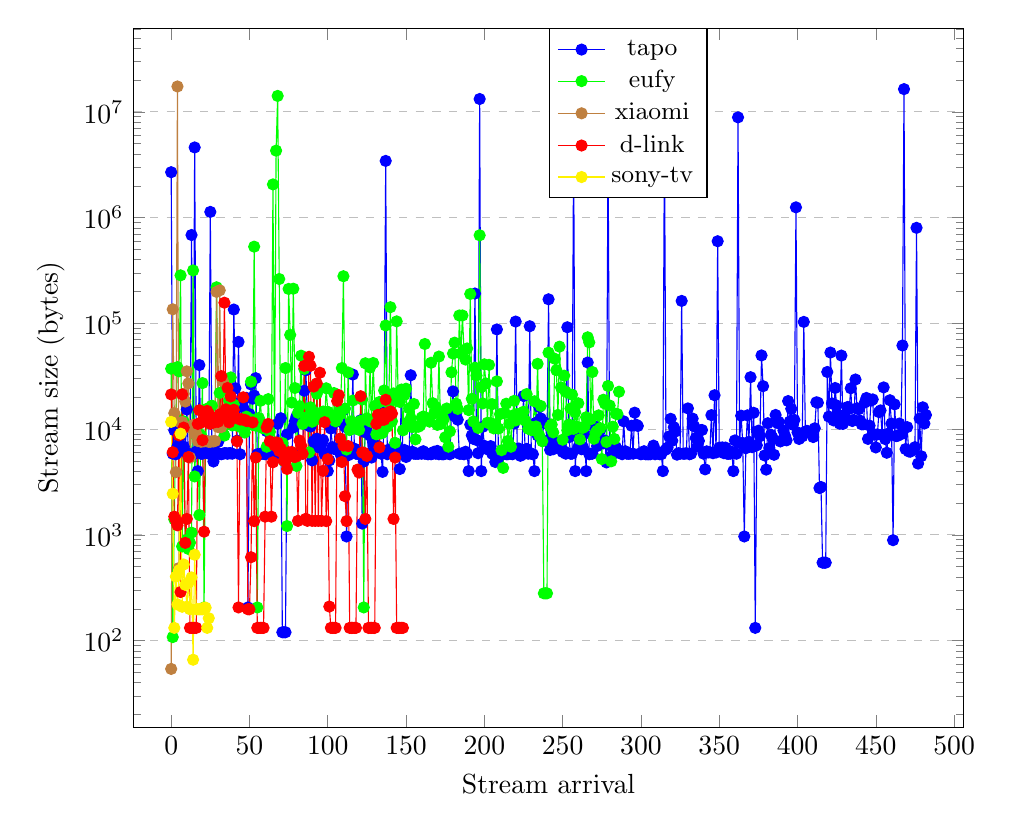
\begin{tikzpicture}[]
\begin{axis}[
%    title={Time (ms)},
    width=\textwidth,           % span entire text width
    %height=0.5\textwidth,       % adjust height as needed
    xlabel={Stream arrival},
    ylabel={ Stream size (bytes)},
    %xmin=0, xmax=11,
    %ymin=0, ymax=60000,
    %xtick={0,1,2,3,4,5,6,7,8,9,10,11},
    %ytick={0, 500,1000,5000,10000,15000,20000,25000,30000,35000,40000,45000,50000,55000,60000},
    legend pos=north west,
    ymajorgrids=true,
	enlarge x limits=0.05,
    grid style=dashed,
    ymode = log,
    %every axis plot/.append style={thick}
    legend style={
        at={(0.5,1)},        % position: (x,y) relative to axis (1,1) is top-right)
        anchor=north west,    % anchor of the legend box
        draw=black,           % optional: add border
        fill=white,           % optional: fill color
        font=\small           % optional: adjust font size
        }
]















 
\addplot[
    color=blue,
    mark=*,
    ]
coordinates {
(0, 2688235)
(1, 5855)
(2, 9757)
(3, 5789)
(4, 6889)
(5, 8522)
(6, 8618)
(7, 6459)
(8, 6841)
(9, 6096)
(10, 15333)
(11, 5789)
(12, 5789)
(13, 684715)
(14, 5789)
(15, 4609320)
(16, 6115)
(17, 4009)
(18, 40348)
(19, 5855)
(20, 5855)
(21, 7327)
(22, 6274)
(23, 6548)
(24, 5855)
(25, 1132768)
(26, 5855)
(27, 4941)
(28, 5996)
(29, 5855)
(30, 7571)
(31, 5855)
(32, 5789)
(33, 5855)
(34, 5921)
(35, 5921)
(36, 5855)
(37, 5921)
(38, 5921)
(39, 5855)
(40, 135183)
(41, 24376)
(42, 7782)
(43, 66810)
(44, 5789)
(45, 19034)
(46, 16080)
(47, 11280)
(48, 19752)
(49, 206)
(50, 13861)
(51, 26417)
(52, 19391)
(53, 20753)
(54, 30333)
(55, 5789)
(56, 5789)
(57, 5855)
(58, 5855)
(59, 5855)
(60, 5789)
(61, 9564)
(62, 6058)
(63, 5789)
(64, 5855)
(65, 5855)
(66, 5855)
(67, 5855)
(68, 11212)
(69, 5855)
(70, 12679)
(71, 120)
(72, 120)
(73, 120)
(74, 8903)
(75, 5921)
(76, 5855)
(77, 5789)
(78, 10353)
(79, 11865)
(80, 13215)
(81, 12325)
(82, 5855)
(83, 5921)
(84, 5855)
(85, 23058)
(86, 36058)
(87, 12498)
(88, 10736)
(89, 10578)
(90, 5057)
(91, 7685)
(92, 7021)
(93, 8126)
(94, 6723)
(95, 6709)
(96, 7237)
(97, 7886)
(98, 5789)
(99, 5855)
(100, 4009)
(101, 5057)
(102, 10121)
(103, 6757)
(104, 6490)
(105, 11640)
(106, 6473)
(107, 6671)
(108, 5855)
(109, 5855)
(110, 15168)
(111, 10536)
(112, 966)
(113, 5651)
(114, 6820)
(115, 6118)
(116, 32815)
(117, 6537)
(118, 5855)
(119, 5855)
(120, 5789)
(121, 12129)
(122, 1278)
(123, 4941)
(124, 9324)
(125, 10563)
(126, 5789)
(127, 8687)
(128, 5381)
(129, 7496)
(130, 6459)
(131, 6709)
(132, 6907)
(133, 6544)
(134, 5855)
(135, 3943)
(136, 14394)
(137, 3438605)
(138, 5789)
(139, 6404)
(140, 6114)
(141, 5855)
(142, 5789)
(143, 6217)
(144, 7030)
(145, 5789)
(146, 4195)
(147, 23251)
(148, 5855)
(149, 6349)
(150, 5451)
(151, 5789)
(152, 5789)
(153, 32312)
(154, 6114)
(155, 5855)
(156, 5855)
(157, 5855)
(158, 5855)
(159, 5921)
(160, 5855)
(161, 6181)
(162, 5855)
(163, 5855)
(164, 5789)
(165, 5855)
(166, 5789)
(167, 5855)
(168, 6115)
(169, 5855)
(170, 6223)
(171, 5789)
(172, 5855)
(173, 5789)
(174, 5789)
(175, 5855)
(176, 6180)
(177, 5855)
(178, 5789)
(179, 14163)
(180, 22737)
(181, 13268)
(182, 14144)
(183, 12270)
(184, 5855)
(185, 5855)
(186, 5855)
(187, 5789)
(188, 6114)
(189, 5855)
(190, 4009)
(191, 11028)
(192, 8741)
(193, 8094)
(194, 191473)
(195, 7886)
(196, 5921)
(197, 13230348)
(198, 4009)
(199, 10518)
(200, 6955)
(201, 6556)
(202, 6459)
(203, 6655)
(204, 6907)
(205, 5855)
(206, 5789)
(207, 4888)
(208, 87641)
(209, 5346)
(210, 5789)
(211, 5789)
(212, 6245)
(213, 5855)
(214, 5789)
(215, 5789)
(216, 5921)
(217, 5855)
(218, 5789)
(219, 11284)
(220, 104014)
(221, 6490)
(222, 6555)
(223, 5592)
(224, 5724)
(225, 20555)
(226, 6301)
(227, 6505)
(228, 5855)
(229, 93945)
(230, 5855)
(231, 5789)
(232, 4009)
(233, 11489)
(234, 8735)
(235, 16191)
(236, 12639)
(237, 7871)
(238, 11667)
(239, 11329)
(240, 7673)
(241, 168914)
(242, 6353)
(243, 8258)
(244, 6459)
(245, 6841)
(246, 7171)
(247, 7236)
(248, 7525)
(249, 7222)
(250, 6088)
(251, 6172)
(252, 5855)
(253, 91875)
(254, 8382)
(255, 5855)
(256, 5855)
(257, 4903915)
(258, 4009)
(259, 8552)
(260, 6757)
(261, 8258)
(262, 6459)
(263, 6709)
(264, 9027)
(265, 4009)
(266, 42637)
(267, 5789)
(268, 5855)
(269, 5855)
(270, 10707)
(271, 8164)
(272, 6913)
(273, 9516)
(274, 9812)
(275, 7794)
(276, 7328)
(277, 7805)
(278, 4840)
(279, 5028493)
(280, 5373)
(281, 6933)
(282, 5856)
(283, 5922)
(284, 6752)
(285, 6030)
(286, 6024)
(287, 6184)
(288, 5789)
(289, 11849)
(290, 6181)
(291, 5855)
(292, 5855)
(293, 5855)
(294, 10758)
(295, 5855)
(296, 14309)
(297, 11010)
(298, 10710)
(299, 5855)
(300, 5789)
(301, 5855)
(302, 6182)
(303, 5789)
(304, 5789)
(305, 5789)
(306, 5789)
(307, 5921)
(308, 6987)
(309, 5789)
(310, 6182)
(311, 5855)
(312, 5789)
(313, 5789)
(314, 4009)
(315, 6645833)
(316, 6410)
(317, 6685)
(318, 8535)
(319, 12515)
(320, 7761)
(321, 10440)
(322, 9493)
(323, 5736)
(324, 5922)
(325, 5855)
(326, 163083)
(327, 5855)
(328, 5855)
(329, 5921)
(330, 15703)
(331, 5789)
(332, 5855)
(333, 12582)
(334, 10635)
(335, 8244)
(336, 6848)
(337, 7741)
(338, 9754)
(339, 9812)
(340, 5855)
(341, 4165)
(342, 6164)
(343, 6023)
(344, 6045)
(345, 13561)
(346, 5921)
(347, 20918)
(348, 6011)
(349, 598002)
(350, 6676)
(351, 6657)
(352, 6709)
(353, 5922)
(354, 6686)
(355, 5855)
(356, 5855)
(357, 5855)
(358, 6116)
(359, 4009)
(360, 7820)
(361, 5855)
(362, 8873587)
(363, 7404)
(364, 13393)
(365, 7398)
(366, 966)
(367, 6595)
(368, 13499)
(369, 7581)
(370, 30985)
(371, 6752)
(372, 14269)
(373, 132)
(374, 7027)
(375, 9659)
(376, 8557)
(377, 49767)
(378, 25477)
(379, 5640)
(380, 4142)
(381, 11370)
(382, 6625)
(383, 8854)
(384, 8298)
(385, 5719)
(386, 13615)
(387, 11458)
(388, 11697)
(389, 7647)
(390, 7813)
(391, 9710)
(392, 8681)
(393, 7835)
(394, 18425)
(395, 11750)
(396, 15583)
(397, 10999)
(398, 12219)
(399, 1250593)
(400, 9315)
(401, 8073)
(402, 8814)
(403, 8537)
(404, 103260)
(405, 9433)
(406, 9628)
(407, 9502)
(408, 9437)
(409, 9484)
(410, 8412)
(411, 10184)
(412, 17927)
(413, 17783)
(414, 2771)
(415, 2837)
(416, 546)
(417, 546)
(418, 546)
(419, 34702)
(420, 13137)
(421, 52973)
(422, 17517)
(423, 12090)
(424, 24498)
(425, 16731)
(426, 13630)
(427, 11247)
(428, 49601)
(429, 11196)
(430, 13528)
(431, 12342)
(432, 16198)
(433, 15585)
(434, 24341)
(435, 11936)
(436, 12196)
(437, 29472)
(438, 15748)
(439, 15419)
(440, 12020)
(441, 11102)
(442, 11115)
(443, 17876)
(444, 19718)
(445, 8080)
(446, 10801)
(447, 18646)
(448, 19106)
(449, 8915)
(450, 6709)
(451, 8913)
(452, 14483)
(453, 15035)
(454, 8872)
(455, 24809)
(456, 8044)
(457, 5978)
(458, 9083)
(459, 18767)
(460, 11287)
(461, 891)
(462, 17138)
(463, 8588)
(464, 8658)
(465, 11287)
(466, 8939)
(467, 61790)
(468, 16411474)
(469, 6479)
(470, 10446)
(471, 6155)
(472, 6118)
(473, 6342)
(474, 6413)
(475, 6752)
(476, 800763)
(477, 4721)
(478, 12618)
(479, 5544)
(480, 16077)
(481, 11289)
(482, 13598)

  
};





\addplot[
    color=green,
    mark=*,
    ]
    coordinates {
(0, 37247)
(1, 108)
(2, 1401)
(3, 12793)
(4, 38590)
(5, 35193)
(6, 284491)
(7, 778)
(8, 11835)
(9, 778)
(10, 898)
(11, 736)
(12, 844)
(13, 1050)
(14, 316719)
(15, 3570)
(16, 8719)
(17, 8601)
(18, 1540)
(19, 8772)
(20, 27253)
(21, 206)
(22, 7777)
(23, 15608)
(24, 14285)
(25, 11834)
(26, 16666)
(27, 11437)
(28, 12595)
(29, 219418)
(30, 11552)
(31, 22013)
(32, 10736)
(33, 10228)
(34, 8688)
(35, 24216)
(36, 12823)
(37, 18598)
(38, 30844)
(39, 10834)
(40, 17101)
(41, 12453)
(42, 12165)
(43, 10654)
(44, 11856)
(45, 10694)
(46, 11455)
(47, 9280)
(48, 13126)
(49, 12513)
(50, 12535)
(51, 28121)
(52, 10948)
(53, 531537)
(54, 10775)
(55, 206)
(56, 12748)
(57, 18529)
(58, 10264)
(59, 11138)
(60, 10078)
(61, 6816)
(62, 19221)
(63, 9441)
(64, 7510)
(65, 2061571)
(66, 7473)
(67, 4298447)
(68, 14153432)
(69, 262713)
(70, 7356)
(71, 7393)
(72, 5002)
(73, 37801)
(74, 1212)
(75, 211669)
(76, 77788)
(77, 17854)
(78, 212714)
(79, 24487)
(80, 4484)
(81, 14274)
(82, 16491)
(83, 49517)
(84, 11209)
(85, 37047)
(86, 12267)
(87, 13052)
(88, 6023)
(89, 16086)
(90, 11742)
(91, 14558)
(92, 26069)
(93, 21604)
(94, 12576)
(95, 12498)
(96, 12524)
(97, 14662)
(98, 12624)
(99, 24324)
(100, 14593)
(101, 13123)
(102, 12613)
(103, 13358)
(104, 21937)
(105, 11848)
(106, 12597)
(107, 14705)
(108, 13809)
(109, 37802)
(110, 279096)
(111, 15618)
(112, 6409)
(113, 34372)
(114, 9792)
(115, 11847)
(116, 18636)
(117, 10485)
(118, 10122)
(119, 10545)
(120, 9850)
(121, 11964)
(122, 19047)
(123, 206)
(124, 41940)
(125, 12643)
(126, 12086)
(127, 38274)
(128, 11690)
(129, 42212)
(130, 16570)
(131, 8928)
(132, 9509)
(133, 18059)
(134, 9101)
(135, 9248)
(136, 23208)
(137, 95506)
(138, 10543)
(139, 17634)
(140, 142263)
(141, 11867)
(142, 21768)
(143, 7426)
(144, 104481)
(145, 18409)
(146, 18079)
(147, 23667)
(148, 9734)
(149, 21080)
(150, 24102)
(151, 11540)
(152, 15708)
(153, 12654)
(154, 10435)
(155, 17293)
(156, 8001)
(157, 10560)
(158, 10551)
(159, 10847)
(160, 12839)
(161, 13169)
(162, 63838)
(163, 12526)
(164, 12541)
(165, 11765)
(166, 42435)
(167, 17607)
(168, 14105)
(169, 16224)
(170, 10962)
(171, 48557)
(172, 11166)
(173, 13370)
(174, 12374)
(175, 8366)
(176, 15682)
(177, 6821)
(178, 9529)
(179, 34455)
(180, 51853)
(181, 65736)
(182, 17386)
(183, 15532)
(184, 118747)
(185, 51926)
(186, 118779)
(187, 55682)
(188, 45481)
(189, 57941)
(190, 15124)
(191, 189675)
(192, 19339)
(193, 11801)
(194, 38158)
(195, 32099)
(196, 10260)
(197, 680699)
(198, 24974)
(199, 17504)
(200, 40986)
(201, 27038)
(202, 11489)
(203, 40501)
(204, 11406)
(205, 17217)
(206, 10162)
(207, 11054)
(208, 28283)
(209, 10127)
(210, 13844)
(211, 6322)
(212, 4298)
(213, 14238)
(214, 17399)
(215, 7733)
(216, 11219)
(217, 6809)
(218, 13434)
(219, 18502)
(220, 12076)
(221, 13900)
(222, 13347)
(223, 13898)
(224, 14100)
(225, 14602)
(226, 12038)
(227, 21440)
(228, 10103)
(229, 10662)
(230, 9796)
(231, 9850)
(232, 18333)
(233, 10592)
(234, 41437)
(235, 8753)
(236, 16571)
(237, 7679)
(238, 280)
(239, 280)
(240, 280)
(241, 52837)
(242, 10535)
(243, 11046)
(244, 9315)
(245, 46259)
(246, 36103)
(247, 13625)
(248, 60256)
(249, 24738)
(250, 7941)
(251, 32007)
(252, 22526)
(253, 9766)
(254, 11035)
(255, 15657)
(256, 21173)
(257, 10060)
(258, 14468)
(259, 10565)
(260, 17549)
(261, 8002)
(262, 10320)
(263, 10299)
(264, 10619)
(265, 12950)
(266, 73855)
(267, 66101)
(268, 12397)
(269, 34691)
(270, 8102)
(271, 9207)
(272, 9651)
(273, 13502)
(274, 10221)
(275, 5215)
(276, 18963)
(277, 17452)
(278, 7556)
(279, 25581)
(280, 16729)
(281, 4958)
(282, 10537)
(283, 8074)
(284, 13977)
(285, 13876)
(286, 22563)
};

    




\addplot[
    color=brown,
    mark=*,
    ]
    coordinates {
(0, 54)
(1, 135792)
(2, 14164)
(3, 3921)
(4, 17385382)
(5, 486)
(6, 11550)
(7, 11634)
(8, 21571)
(9, 18228)
(10, 35166)
(11, 27089)
(12, 5392)
(13, 10187)
(14, 10954)
(15, 9041)
(16, 9041)
(17, 7720)
(18, 7720)
(19, 7600)
(20, 7666)
(21, 7666)
(22, 7720)
(23, 7666)
(24, 7600)
(25, 7600)
(26, 7666)
(27, 7654)
(28, 7720)
(29, 198616)
(30, 10447)
(31, 205314)
(32, 10447)
(33, 28504)
};













\addplot[
    color=red,
    mark=*,
    ]
    coordinates {
(0, 21277)
(1, 6045)
(2, 1487)
(3, 1363)
(4, 1231)
(5, 8720)
(6, 288)
(7, 21288)
(8, 10336)
(9, 840)
(10, 1415)
(11, 5438)
(12, 132)
(13, 132)
(14, 132)
(15, 132)
(16, 132)
(17, 11203)
(18, 15088)
(19, 11501)
(20, 7866)
(21, 1072)
(22, 13603)
(23, 14868)
(24, 14011)
(25, 11218)
(26, 12220)
(27, 12685)
(28, 11656)
(29, 12393)
(30, 11733)
(31, 13793)
(32, 31720)
(33, 13296)
(34, 156861)
(35, 15379)
(36, 24494)
(37, 11570)
(38, 20385)
(39, 14452)
(40, 15246)
(41, 12856)
(42, 7675)
(43, 206)
(44, 12328)
(45, 12408)
(46, 19990)
(47, 12238)
(48, 11929)
(49, 198)
(50, 198)
(51, 615)
(52, 11572)
(53, 1349)
(54, 5384)
(55, 132)
(56, 132)
(57, 132)
(58, 132)
(59, 132)
(60, 1487)
(61, 10368)
(62, 11206)
(63, 7681)
(64, 1487)
(65, 4859)
(66, 7023)
(67, 7485)
(68, 7417)
(69, 6215)
(70, 6544)
(71, 6085)
(72, 5045)
(73, 4912)
(74, 4199)
(75, 6042)
(76, 5727)
(77, 6078)
(78, 5512)
(79, 5450)
(80, 5534)
(81, 1357)
(82, 7790)
(83, 6982)
(84, 5848)
(85, 39652)
(86, 1420)
(87, 1357)
(88, 48281)
(89, 39724)
(90, 1357)
(91, 25247)
(92, 1357)
(93, 27079)
(94, 1357)
(95, 34122)
(96, 1357)
(97, 4032)
(98, 11618)
(99, 1349)
(100, 5198)
(101, 210)
(102, 132)
(103, 132)
(104, 132)
(105, 132)
(106, 18444)
(107, 20975)
(108, 8152)
(109, 4886)
(110, 6994)
(111, 2322)
(112, 1349)
(113, 6910)
(114, 132)
(115, 132)
(116, 132)
(117, 132)
(118, 132)
(119, 4138)
(120, 3886)
(121, 20468)
(122, 6005)
(123, 5991)
(124, 1415)
(125, 5576)
(126, 132)
(127, 132)
(128, 132)
(129, 132)
(130, 132)
(131, 11213)
(132, 13646)
(133, 6718)
(134, 12170)
(135, 13905)
(136, 12264)
(137, 18954)
(138, 14166)
(139, 13290)
(140, 14726)
(141, 14023)
(142, 1415)
(143, 5384)
(144, 132)
(145, 132)
(146, 132)
(147, 132)
(148, 132)
};




















\addplot[
    color=yellow,
    mark=*,
    ]
    coordinates {
(0, 11705)
(1, 2449)
(2, 132)
(3, 403)
(4, 220)
(5, 462)
(6, 9060)
(7, 209)
(8, 525)
(9, 337)
(10, 209)
(11, 353)
(12, 198)
(13, 396)
(14, 66)
(15, 648)
(16, 198)
(17, 198)
(18, 198)
(19, 198)
(20, 198)
(21, 205)
(22, 205)
(23, 132)
(24, 163)
};











\legend{tapo, eufy, xiaomi, d-link, sony-tv}
\end{axis}
\end{tikzpicture}
}
 \caption[justification=centering]{Stream size.}
  \label{fig:stream_size}
\end{figure}


\begin{comment}
    

\section{Entropy}

Figure \ref{fig:device_comparison} contains six time-series subplots (a-f), each showing entropy measures computed for a sequence of update-related network sessions from a single device/platform. The x-axis in every subplot is the session index (consecutive update-related sessions captured for that device); the x-axis length differs per device because the number of sessions varies. 
The y-axis is normalized entropy (range 0.00-1.00). 
Each plot overlays three entropy metrics: Shannon (blue), Rényi (red), and Tsallis (yellow). 
The legend in each subplot identifies these three traces.
To describe these panel-by-panel observations:
\begin{itemize}
    \item [\textbullet]
    (a) appletv: Shannon and Rényi entropies sit roughly in the 0.65-0.85 band and show gentle, correlated oscillations across sessions; Rényi is consistently slightly lower than Shannon. 
    Tsallis is much higher ($\approx$0.90-0.99) and relatively flat, indicating a systematic offset between Tsallis and the other two metrics for this device.

    \item [\textbullet]
    (b) roku-tv: Entropy traces show larger short-term variability, especially at small session indices where all three metrics fluctuate sharply. After the initial volatility, Shannon and Rényi settle into a band around 0.50-0.70, while Tsallis remains high but exhibits larger swings than in (a), briefly approaching 1.0 at several points.

    \item [\textbullet]
    (c) fire-tv: All three metrics are relatively stable with Shannon and Rényi around 0.65-0.80 and Tsallis near 0.95-1.00. The traces are closely correlated, with modest session-to-session variation and no large outliers.
    
    \item [\textbullet]
    (d) samsung-tv: Shannon and Rényi gradually trend toward slightly lower values ($\approx$0.60-0.75) with a few small spikes; Tsallis again remains near the top of the scale ($\approx$0.93-0.99). A localized increase appears in the later sessions.

    \item [\textbullet]
    (e) echo-dot: Shannon and Rényi typically lie in the 0.55-0.75 range; Rényi shows more pronounced short dips than Shannon. Tsallis is near 0.95 for most of the sequence but drops sharply near the very end (a clear deviation from the earlier pattern).

    \item [\textbullet]
    (f) echo-plus: Shannon is fairly stable around 0.70-0.80. Rényi displays the greatest volatility among all devices, with multiple low spikes (down toward 0.30-0.40) interspersed with higher values. 
    Tsallis remains high and steady ($\approx$0.90-0.98).

\end{itemize}

To summarize,
the three entropy measures produce distinct numerical ranges for the same sessions: Tsallis consistently returns the highest values, Shannon intermediate, and Rényi the lowest (and most volatile in some cases). 
This is expected because these metrics emphasize distributional features differently; the visual separation highlights the value of comparing multiple entropy formulations rather than relying on a single entropy measure.






For the analyzed IoT device, each device exhibits a characteristic entropy profile (level, volatility, and occasional abrupt changes). 
Such profiles can be used to (a) flag anomalous sessions, (b) distinguish device families,  or (c) infer when a session is highly encrypted versus plaintext (e.g., sustained high entropy is consistent with encrypted/pseudo-random payloads).
On the anomalies and session-level diagnostics. 
Sharp drops or spikes - for example, the end-of-sequence drop in Tsallis for echodot, or the low Rényi spikes in echoplus - merit inspection: they may indicate transitions between encrypted and plaintext transfers, short control packets, or extraction artifacts.










Table ?? presents the entropy analysis results for update-related sessions across six IoT devices.  
The reported values represent the average of session-level entropy measures, aggregated per device,
providing complementary perspectives on the randomness and potential encryption of the payload data.
Across all devices, Tsallis entropy values are consistently the highest.
This suggests that Tsallis entropy is more sensitive in detecting high-randomness distributions in the payload, making it an effective indicator of encrypted traffic. Shannon entropy results show moderate-to-high values, with apple-tv and  fire-tv   exhibiting the strongest indications of encrypted traffic. 
Rényi entropy values are consistently lower than both Shannon and Tsallis, which may reflect its sensitivity to dominant probability distributions in the data.

%In terms of device-specific trends, Fire TV and Apple TV show the strongest alignment across all three entropy metrics, supporting the inference that these devices handle a greater proportion of encrypted update-related traffic. Roku TV consistently reports the lowest values across the three metrics, indicating that its update-related sessions may include a higher proportion of unencrypted or weakly encrypted traffic. Samsung TV, Echo Dot, and Echo Plus fall between these two extremes, showing moderate entropy values but with Tsallis approaching near-maximum for all.




\end{comment}

    






\begin{comment}
    












%%%%%%%%%%%%%%%%%55
%%%%%%%%%%%%%%%%5


\begin{figure*}[htb]
    \centering
    % --- First row: 2 figures ---
    \begin{subfigure}{0.48\textwidth}
        \centering
        \includegraphics[width=\linewidth]{fig/tapo_entropy_plot.pdf}
        \caption{Tapo entropy}
    \end{subfigure}
    %\hfill
    \begin{subfigure}{0.48\textwidth}
        \centering
        \includegraphics[width=\linewidth]{fig/dlink_entropy_plot.pdf}
        \caption{Dlink entropy}
    \end{subfigure}

    % --- Second row: 3 figures ---
    \begin{subfigure}{0.48\textwidth}
        \centering
        \includegraphics[width=\linewidth]{fig/eufy_entropy_plot.pdf}
        \caption{Eufy entropy}
    \end{subfigure}
    %\hfill
    \begin{subfigure}{0.48\textwidth}
        \centering
        \includegraphics[width=\linewidth]{fig/xiaomi_entropy_plot.pdf}
        \caption{Xiaomi entropy}
    \end{subfigure}
   % \hfill
   % \begin{subfigure}{0.32\textwidth}
    %    \centering
     %   \includegraphics[width=\linewidth]{fig/sony_entropy_plot.pdf}
      %  \caption{Sony-tv entropy}
    %\end{subfigure}

    \caption{Entropy plots for controlled experiments.}
    \label{fig:five-entropy}
\end{figure*}






\end{comment}


\begin{comment}
    
%%%%%%%%%%%%%%%%%%%%%%%
%%%%%%%%%%%%%%

\begin{figure}
    \centering
    % First row
    \begin{subfigure}[b]{0.48\textwidth}
        \centering
        \includegraphics[width=\textwidth]{fig/appletv.pdf}
        \caption{appletv}
        \label{fig:appletv}
    \end{subfigure}
    \begin{subfigure}[b]{0.48\textwidth}
        \centering
        \includegraphics[width=\textwidth]{fig/rokutv.pdf}
        \caption{rokutv}
        \label{fig:rokutv}
    \end{subfigure}
    
    %\vspace{0.5em} % optional vertical spacing between rows



    % Second row
    \begin{subfigure}[b]{0.47\textwidth}
        \centering
        \includegraphics[width=\textwidth]{fig/firetv.pdf}
        \caption{firetv}
        \label{fig:firetv}
    \end{subfigure}
    \begin{subfigure}[b]{0.47\textwidth}
        \centering
        \includegraphics[width=\textwidth]{fig/samsungtv.pdf}
        \caption{samsungtv}
        \label{fig:samsungtv}
    \end{subfigure}

    

    \begin{subfigure}[b]{0.49\textwidth}
        \centering
        \includegraphics[width=\textwidth]{fig/echodot.pdf}
        \caption{echodot}
        \label{fig:echodot}
    \end{subfigure}
    \begin{subfigure}[b]{0.49\textwidth}
        \centering
        \includegraphics[width=\textwidth]{fig/echoplus.pdf}
        \caption{echoplus}
        \label{fig:echoplus}
    \end{subfigure}


    \caption{Session-wise comparison of  entropy metrics (Shannon-blue, Rényi-red, Tsallis-yellow) for update-related network traffic on six IoT platforms.
    Plots show device-specific entropy levels, inter-session variability, and occasional abrupt deviations that may indicate changes in payload structure or encryption state.}
    \label{fig:device_comparison}
\end{figure}


\end{comment}


\begin{comment}

\section{Retrospective findings}




We further extracted the update-related interaction event \cite{10.1007/978-3-031-30122-3_25} as shown in Figure \ref{fig:update-event}. 
We can see that Andoriad and Alexa has the highest update interaction event. 
This is due to a combination of 9 Android events (\emph{android\_lan\_off: 583,
android\_lan\_on: 570,
android\_lan\_menu: 216,
android\_lan\_remote: 76,
android\_wan\_recording: 2,
android\_lan\_watch: 2,
android\_wan\_watch: 1,
android\_lan\_recording: 1, 
android\_lan\_photo: 1}),  
and a combination of 4 
Alex events (\emph{alexa\_off: 147,
alexa\_on: 146,
alexa\_dim: 144,
alexa\_color: 73}).







\begin{figure}
    \centering
    \includegraphics[width=0.8\linewidth]{fig/heatmap_event.png}
    \caption{Update-related interaction events.}
    \label{fig:update-event}
\end{figure}








\begin{figure}[htbp]
    \centering
    \includegraphics[width=1\linewidth]{fig/cwe_counts_top6.png}
    \caption{CWE counts top6}
    \label{fig:cwe_counts_top6}
\end{figure}    
\end{comment}






